\RequirePackage{fix-cm}
\documentclass[11pt,a4paper]{article}
\usepackage[utf8]{inputenc}
\usepackage[margin=2cm]{geometry}
\usepackage{amsmath,amssymb,mathtools}
\usepackage{booktabs,array,multirow}
\usepackage[most]{tcolorbox}
\usepackage{enumitem}
\setlist[itemize]{itemsep=1pt, topsep=2pt, label=$\bullet$}
\setlist[enumerate]{itemsep=1pt, topsep=2pt}
\usepackage{listings}
\usepackage{tikz}
\usetikzlibrary{arrows.meta,positioning,shapes.geometric,calc,fit}
\usepackage{pgfplots}
\pgfplotsset{compat=1.18}
% ---- matplotlib look for the plots drawn by LaTeX (no image files needed)
\definecolor{tabblue}{HTML}{1F77B4}\definecolor{taborange}{HTML}{FF7F0E}
\definecolor{tabgreen}{HTML}{2CA02C}\definecolor{tabred}{HTML}{D62728}
\pgfplotsset{mpl/.style={scale only axis, axis line style={black,line width=0.8pt},
  tick style={black,line width=0.8pt}, tick align=outside, xtick pos=bottom, ytick pos=left,
  major tick length=3.5pt, tick label style={font=\fontsize{10}{12}\selectfont\sffamily},
  legend cell align=left, legend style={draw=black!20, rounded corners=2pt, fill=white, fill opacity=0.8, text opacity=1},
  legend image code/.code={\draw[#1] (0pt,0pt) -- (22pt,0pt);}},
  mplgrid/.style={grid=major, major grid style={black!30, line width=0.8pt, dash pattern=on 2.96pt off 1.28pt}},
  mplmark/.style={legend image code/.code={\draw[mark repeat=2,mark phase=2,##1] plot coordinates {(0pt,0pt) (11pt,0pt) (22pt,0pt)};}}}
\tikzset{mpldash/.style={dash pattern=on 3.7pt off 1.6pt}, mpldot/.style={dash pattern=on 1pt off 1.65pt}}
% ---- flowcharts
\tikzset{
  fcbox/.style={rectangle, draw=DefBlue, line width=0.8pt, fill=DefBlue!4, align=flush center, font=\small, inner sep=3pt, minimum height=8mm},
  fcdec/.style={diamond, aspect=2.2, draw=LemRed, line width=0.8pt, fill=LemRed!4, align=flush center, font=\small, inner sep=2pt},
  fcterm/.style={rectangle, rounded corners=3mm, draw=AnsGreen, line width=0.8pt, fill=AnsGreen!8, align=flush center, font=\small, inner sep=3pt, minimum height=7mm},
  fcerr/.style={rectangle, rounded corners=3mm, draw=tabred, line width=0.8pt, fill=tabred!6, align=flush center, font=\small, inner sep=3pt, minimum height=7mm},
  fcplot/.style={rectangle, draw=taborange, line width=0.8pt, fill=taborange!7, align=flush center, font=\small, inner sep=3pt, minimum height=8mm},
  fcarr/.style={-{Stealth[length=2.2mm,width=1.8mm]}, line width=0.8pt},
  fcloop/.style={draw=CodeGray, line width=0.6pt, dashed, rounded corners=2mm, inner sep=2.5mm},
  fclab/.style={font=\footnotesize, text=CodeGray},
}
\usepackage{caption}
\usepackage{hyperref}
\hypersetup{colorlinks=true,linkcolor=black,citecolor=black,urlcolor=black,
  pdftitle={Financial Processes -- Homework 3: digital options},pdfauthor={Carlos Chipantiza}}
\usepackage{needspace}
\captionsetup{hypcap=false}
\frenchspacing
\emergencystretch=3em

\definecolor{DefBlue}{RGB}{16,64,120}
\definecolor{LemRed}{RGB}{170,30,40}
\definecolor{ThmPurple}{RGB}{95,40,130}
\definecolor{AnsGreen}{RGB}{20,120,70}
\definecolor{CodeGray}{RGB}{110,110,110}
\definecolor{FIX}{RGB}{20,120,70}

\newcounter{defn}\newcounter{lemn}\newcounter{thmn}\newcounter{corn}
\newtcolorbox{defbox}[1]{enhanced,colback=white,colframe=DefBlue,boxrule=0.8pt,arc=1mm,left=2mm,right=2mm,top=1.5mm,bottom=1.5mm,
  before upper={\refstepcounter{defn}\noindent\textbf{Definition \thedefn} (#1).\par\smallskip}}
\newtcolorbox{lembox}[1]{enhanced,colback=white,colframe=LemRed,boxrule=0.8pt,arc=1mm,left=2mm,right=2mm,top=1.5mm,bottom=1.5mm,
  before upper={\refstepcounter{lemn}\noindent\textbf{Lemma \thelemn} (#1).\par\smallskip}}
\newtcolorbox{corbox}[1]{enhanced,colback=white,colframe=LemRed,boxrule=0.8pt,arc=1mm,left=2mm,right=2mm,top=1.5mm,bottom=1.5mm,
  before upper={\refstepcounter{corn}\noindent\textbf{Corollary \thecorn} (#1).\par\smallskip}}
\newtcolorbox{thmbox}[1]{enhanced,colback=white,colframe=ThmPurple,boxrule=0.8pt,arc=1mm,left=2mm,right=2mm,top=1.5mm,bottom=1.5mm,
  before upper={\refstepcounter{thmn}\noindent\textbf{Theorem \thethmn} (#1).\par\smallskip}}
\newtcolorbox{stmbox}[1]{enhanced,colback=white,colframe=CodeGray,boxrule=0.8pt,arc=1mm,left=2mm,right=2mm,top=1.5mm,bottom=1.5mm,
  before upper={\noindent\textbf{Statement of the professor} (#1).\par\smallskip}}
\newtcolorbox{ansboxenv}{enhanced,colback=AnsGreen!6,colframe=AnsGreen,boxrule=0.8pt,arc=1mm,left=2mm,right=2mm,top=1.5mm,bottom=1.5mm}
\newcommand{\ansbox}[1]{\begin{ansboxenv}#1\end{ansboxenv}}
\newcommand{\subhead}[1]{\par\medskip\noindent{\large\bfseries #1}\par\smallskip\noindent\ignorespaces}
\newcommand{\step}[1]{\par\smallskip\noindent\textbf{#1}\enspace\ignorespaces}

% ---- code that can be copied from the PDF and pasted into Python:
% every space is a real character (an invisible glyph mapped to U+0020), no line
% numbers, no line breaks inside a line, straight quotes.
\input{glyphtounicode}
\pdfglyphtounicode{visiblespace}{0020}
\pdfgentounicode=1
\makeatletter
\def\lst@visiblespace{{\color{white}\char32}}
\makeatother
\lstdefinestyle{py}{language=Python,basicstyle=\ttfamily\footnotesize,keywordstyle=\color{DefBlue},
  commentstyle=\color{CodeGray},stringstyle=\color{black},showspaces=true,showstringspaces=false,
  frame=single,rulecolor=\color{CodeGray},numbers=none,
  breaklines=false,columns=fixed,basewidth=0.5em,keepspaces=true,tabsize=4,xleftmargin=0.4em,framexleftmargin=0.4em,
  captionpos=t,literate={\$}{{\char36}}1 {'}{{\char13}}1 {`}{{\char18}}1}
\lstdefinestyle{prof}{style=py,basicstyle=\ttfamily\fontsize{6.6}{7.8}\selectfont}
\lstdefinestyle{pysmall}{style=py,basicstyle=\ttfamily\fontsize{7.6}{9}\selectfont}
\lstdefinestyle{out}{basicstyle=\ttfamily\footnotesize,columns=fixed,basewidth=0.5em,showspaces=true,
  frame=leftline,framerule=1.2pt,rulecolor=\color{FIX},numbers=none,xleftmargin=0.8em,framexleftmargin=0.4em,
  breaklines=false,captionpos=t}
\captionsetup[lstlisting]{labelformat=empty,font={footnotesize,sf},justification=raggedright,singlelinecheck=false,skip=2pt}
\captionsetup[figure]{font=small}
\newcommand{\Et}{\tilde{E}}
\newcommand{\ul}{u_{\text{left}}}
\newcommand{\ur}{u_{\text{right}}}

\tikzset{
  inh/.style={-{Triangle[open,length=2.6mm,width=2.6mm]}, line width=0.8pt, CodeGray},
  usesa/.style={-{Stealth[length=2mm]}, line width=0.8pt, CodeGray},
  ghostb/.style={opacity=0.35, dashed},
  newb/.style={line width=1.6pt, label={[font=\tiny\bfseries, text=white, fill=taborange, inner sep=1.5pt]north east:NEW}},
  blab/.style={font=\scriptsize\itshape, fill=white, inner sep=1pt, align=center},
  lno/.style={font=\scriptsize\color{CodeGray}},
}
\newcommand{\Q}{\mathbb{Q}}
\newcommand{\ind}{\mathbf{1}}
\newcommand{\DF}{e^{-r\tau}}
\newcommand{\pos}[1]{\left(#1\right)^{+}}

\renewcommand{\subhead}[1]{\par\medskip\needspace{8\baselineskip}\noindent{\large\bfseries #1}\par\smallskip\noindent\ignorespaces}
\newcolumntype{L}[1]{>{\raggedright\arraybackslash}p{#1}}
% Block diagrams of the homework: which blocks exist after each piece of code.
% stage 0: library copied from the solution folder; 1: EuropeanDigitalContract; 2: EuropeanDigitalAnalyticPricer;
% 3: digital unit tests; 4: Q2 figure script.
\newcommand{\hwstage}[2]{%
  \ifnum#1<#2\relax\tikzset{st#2/.style={ghostb},ast#2/.style={opacity=0.25},atx#2/.style={opacity=0.25}}%
  \else\ifnum#1=#2\relax\tikzset{st#2/.style={newb},ast#2/.style={draw=taborange},atx#2/.style={text=taborange!80!black}}%
  \else\tikzset{st#2/.style={},ast#2/.style={},atx#2/.style={}}\fi\fi}
\newcommand{\hwBlocksPic}[1]{%
\begin{tikzpicture}[every node/.style={font=\footnotesize}]
\hwstage{#1}{1}\hwstage{#1}{2}\hwstage{#1}{3}\hwstage{#1}{4}
% library of Lecture 5 (always there)
\node[fcbox, font=\footnotesize, text width=3.0cm] (md) at (0,0) {\textbf{MarketModel}\\ $S$, $\sigma$, $r$, \texttt{calc\_df}};
\node[fcbox, font=\footnotesize, text width=3.0cm, draw=taborange, fill=taborange!6] (ct) at (6.3,1.9) {\textbf{Contract} (ABC)};
\node[fcbox, font=\footnotesize, text width=3.0cm, draw=taborange, fill=taborange!6] (ec) at (4.2,0) {\textbf{European-}\\\textbf{Contract}};
\node[fcbox, font=\footnotesize, text width=3.0cm, draw=AnsGreen, fill=AnsGreen!6] (pr) at (6.3,-2.3) {\textbf{Pricer} (ABC)};
\node[fcbox, font=\footnotesize, text width=3.2cm, draw=AnsGreen, fill=AnsGreen!6] (ep) at (4.2,-4.4) {\textbf{EuropeanAnalytic-}\\\textbf{Pricer}};
\node[fcbox, font=\footnotesize, text width=3.1cm, draw=CodeGray, fill=CodeGray!6] (tp) at (12.75,-0.3) {\textbf{TestPutCallParity}\\ (lecture, 24 cases)};
% new blocks
\node[fcbox, font=\footnotesize, text width=3.0cm, draw=taborange, fill=taborange!6, st1] (dc) at (8.4,0) {\textbf{EuropeanDigital-}\\\textbf{Contract}};
\node[fcbox, font=\footnotesize, text width=3.0cm, draw=AnsGreen, fill=AnsGreen!6, st2] (dp) at (8.4,-4.4) {\textbf{EuropeanDigital-}\\\textbf{AnalyticPricer}};
\node[fcbox, font=\footnotesize, text width=3.1cm, draw=CodeGray, fill=CodeGray!6, st3] (td) at (12.75,-2.3) {\textbf{digital tests} (Q1)\\ 103 cases};
\node[fcbox, font=\footnotesize, text width=3.1cm, draw=taborange, fill=taborange!6, st4] (fg) at (12.75,-4.4) {\textbf{Q2 figure}\\ \texttt{q2\_bull\_spread.py}};
% connections of the lecture
\draw[inh] (ec.north) -- (ec.north |- ct.south);
\draw[inh] (ep.north) -- (ep.north |- pr.south);
\draw[usesa] (md) |- node[blab, pos=0.75, above] {\texttt{self.model}} (pr.west);
\draw[usesa] (ec.south) -- node[blab, left=1pt, pos=0.4] {\texttt{self.contract}} (pr.north west);
\draw[usesa] (tp.south west) -- node[blab, above, sloped] {checks} (pr.north east);
% new connections
\draw[inh, ast1] (dc.north) -- (dc.north |- ct.south);
\draw[inh, ast2] (dp.north) -- (dp.north |- pr.south);
\draw[usesa, ast2] (dc.south) -- (pr.north east -| dc.south);
\draw[usesa, dashed, ast2] (dp.west) -- node[blab, atx2, above] {$d_1,d_2$} (ep.east);
\draw[usesa, ast3] (td) -- node[blab, atx3, above, sloped] {tests} (dp.north east);
\draw[usesa, ast4] (fg) -- node[blab, atx4, above] {digital} (dp);
\draw[usesa, ast4] (fg.south) -- ++(0,-0.55) -| node[blab, atx4, pos=0.25, below] {spread legs: LONG call $K$, SHORT call $K+h$} (ep.south);
\end{tikzpicture}}
\newcommand{\hwBlocks}[2]{%
\begin{center}\begin{minipage}{\linewidth}\centering
\hwBlocksPic{#1}
\captionof{figure}{Blocks after #2. Bold with NEW: created by this code; faded: still to come. Open triangle: inherits from; plain arrow: uses; dashed: reuses the static $d_1$, $d_2$.}
\label{fig:blk#1}
\end{minipage}\end{center}}

\begin{document}
\noindent Name: Carlos Chipantiza \hfill Neptun code: EACN90\\
\noindent Financial Processes (BMETE95MM14), BME, Fall 2026 \hfill course id: 54932fw\\[2pt]
{\large\textbf{Homework 3 (Lecture 5): Digital options}}\\[2pt]
\noindent\rule{\textwidth}{0.4pt}

\noindent\textbf{Remark.} The results used are stated in boxes and cited by number; results of the lectures are quoted with their cell, the few new ones are short, proved here, and have a reference (list at the end). The code shown is an exact copy of the files and every number is printed by it (files \texttt{*.out}). Files: the library of Lecture 5 (\texttt{solution} folder: \texttt{contract.py}, \texttt{market\_data.py}, \texttt{model.py}, \texttt{pricer.py}, \texttt{test\_pricer.py}) with the NEW CODE added at the end of \texttt{contract.py}, \texttt{pricer.py} and \texttt{test\_pricer.py}; the runs \texttt{q1\_digital\_demo.py} (Q1) and \texttt{q2\_bull\_spread.py} (Q2, with \texttt{my\_plotter} of Homework~1, file \texttt{plotter.py}); the notebooks \texttt{3\_HW\_EXE\_1} (Q1) and \texttt{3\_HW\_EXE\_2} (Q2) with the same code. After each piece of code a block diagram shows how the library grows. Running example (the market of the library): \texttt{BLUECHIP\_BANK}, $S=130.17$, $\sigma=0.381$, $r=0.05$; $K=130$, $T=1$.

\subhead{1. The assignment.}
\begin{stmbox}{\texttt{notebook\_building\_blocks.ipynb}, cell 19}
\emph{Create a new folder under QuantCourseBP\textbackslash homeworks and copy over the content of this lecture's solution folder to start with.}
\begin{enumerate}
\item \emph{Get familiar with digital options and implement EuropeanDigitalContract and EuropeanDigitalAnalyticPricer (fair value and greeks) in the library. Implement unit test for fair value using pytest.} \textbf{(12 points)}
\item \emph{Get familiar with bull spread options and by utilizing EuropeanDigitalAnalyticPricer and EuropeanAnalyticPricer, create a figure to visualize that a digital call option can be thought of as a limit of bull spread call options.} \textbf{(8 points)}
\end{enumerate}
\end{stmbox}

% =====================================================================
\subhead{2. The problem.}
\begin{center}\small
\renewcommand{\arraystretch}{1.25}
\begin{tabular}{@{}L{0.2\textwidth}L{0.42\textwidth}L{0.32\textwidth}@{}}
\toprule
To build & What it must do & Lecture 5 pattern it follows\\
\midrule
\texttt{EuropeanDigital-}\newline\texttt{Contract} & store underlying, CALL/PUT, LONG/SHORT, $K$, $T$; \texttt{payoff} $=\pm\ind\{S_T>K\}$ or $\pm\ind\{S_T<K\}$ & \texttt{EuropeanContract} (\texttt{contract.py})\\
\texttt{EuropeanDigital-}\newline\texttt{AnalyticPricer} & fair value and $\Delta,\Gamma$, vega, $\Theta$, $\rho$ (closed form), times \texttt{direction} & \texttt{EuropeanAnalyticPricer} (\texttt{pricer.py})\\
unit test (Q1) & fair value correct for several stocks, strikes, expiries & \texttt{TestPutCallParity} (\texttt{test\_pricer.py})\\
figure (Q2) & bull spreads $\to$ digital call, with both pricers & plots of Homework~1 (\texttt{plotter.py})\\
\bottomrule
\end{tabular}
\end{center}
\noindent The only mathematics needed: the Black--Scholes price of the digital and its five Greeks (Section 3). Everything else is code in the style of the lecture.

% =====================================================================
\subhead{3. Results used.}
\noindent\emph{From the lectures.}

\begin{defbox}{Digital (cash-or-nothing) option; Hull [4], ``Binary options''}
With strike $K$ and expiry $T$, the \emph{digital call} pays $1$ at $T$ if $S_T>K$ and $0$ otherwise; the \emph{digital put} pays $1$ if $S_T<K$:
\begin{equation}\label{eq:dig}
V_T^{\mathrm{dc}}=\ind\{S_T>K\},\qquad V_T^{\mathrm{dp}}=\ind\{S_T<K\}.
\end{equation}
The lecture only names it (``get familiar with digital options''), so the definition is taken from [4].
\end{defbox}

\begin{defbox}{Bull call spread; Hull [4], ``Bull spreads''}
Long one call with strike $K_1$ and short one call with strike $K_2>K_1$, same expiry. Payoff: $\pos{S_T-K_1}-\pos{S_T-K_2}$, i.e.\ $0$ below $K_1$, linear between, $K_2-K_1$ above $K_2$.
\end{defbox}

\begin{thmbox}{Black--Scholes call and put; Lecture 3, cell 37; Lecture 5, cells 5--6}
With $\tau=T-t$ and $N$ the standard normal cdf,
\begin{equation}\label{eq:bs}
c=S\,N(d_1)-K\DF N(d_2),\qquad p=K\DF N(-d_2)-S\,N(-d_1),
\end{equation}
\begin{equation}\label{eq:d}
d_1=\frac{\ln(S/K)+(r+\sigma^2/2)\tau}{\sigma\sqrt\tau},\qquad d_2=d_1-\sigma\sqrt\tau .
\end{equation}
In the library: \texttt{EuropeanAnalyticPricer} with \texttt{calc\_d1}, \texttt{calc\_d2} (static).
\end{thmbox}

\begin{thmbox}{Black--Scholes PDE; Lecture 3, cells 34--37}
The price $f(t,S)$ of every derivative on the stock satisfies
\begin{equation}\label{eq:pde}
f'_t+\tfrac12\sigma^2S^2f''_{SS}+rSf'_S-rf=0,
\end{equation}
with the payoff as the condition at $t=T$ (``we know the payoff at time $T$'').
\end{thmbox}

\begin{thmbox}{Same payoff, same price; Lecture 3, cells 28--30; Lecture 5, cell 6}
Two portfolios with the same payoff in every state have the same price today (no arbitrage); this gives put--call parity $f=c-p$. In particular $1$ paid surely at $T$ costs $\DF$ today (the bond in $f=S-K\DF$).
\end{thmbox}

\noindent\emph{New, short results} (proved here; references [4], [5]).

\begin{lembox}{Dominance; from Theorem 3 (no arbitrage); [4], [5]}
If two payoffs satisfy $V_T^A\ge V_T^B$ in every state, then their prices satisfy $V^A\ge V^B$.
\end{lembox}
\noindent\emph{Proof.} If $V^A<V^B$: sell $B$, buy $A$, keep $V^B-V^A>0$; at $T$ the position pays $V_T^A-V_T^B\ge0$. A sure gain at no risk is an arbitrage, excluded in Lecture 3 (cell 33). \hfill$\square$

\begin{lembox}{A Black--Scholes identity; algebra on \eqref{eq:d}}
With $\varphi=N'$ the normal density,
\begin{equation}\label{eq:id}
S\,\varphi(d_1)=K\DF\,\varphi(d_2).
\end{equation}
\end{lembox}
\noindent\emph{Proof.} By levels, using $d_2=d_1-\sigma\sqrt\tau$ and \eqref{eq:d}:
\begin{align*}
\frac{\varphi(d_2)}{\varphi(d_1)}&=e^{(d_1^2-d_2^2)/2} && \text{(definition of $\varphi$)}\\
&=e^{(d_1-d_2)(d_1+d_2)/2} && \text{(difference of squares)}\\
&=e^{\sigma\sqrt\tau\,(2d_1-\sigma\sqrt\tau)/2} && \text{($d_1-d_2=\sigma\sqrt\tau$)}\\
&=e^{\ln(S/K)+r\tau} && \text{(insert $d_1$ from \eqref{eq:d})}\\
&=\frac{S}{K\DF}. && \hfill\square
\end{align*}

\begin{lembox}{Strike derivatives; from Theorem 1 and Lemma 2; Breeden--Litzenberger [6]}
\begin{equation}\label{eq:dK}
\frac{\partial c}{\partial K}=-\DF N(d_2),\qquad \frac{\partial p}{\partial K}=\DF N(-d_2).
\end{equation}
\end{lembox}
\noindent\emph{Proof.} Both $d_1$ and $d_2$ depend on $K$ with $\partial d_1/\partial K=\partial d_2/\partial K$. Differentiate \eqref{eq:bs}:
\begin{align*}
\frac{\partial c}{\partial K}&=S\varphi(d_1)\frac{\partial d_1}{\partial K}-\DF N(d_2)-K\DF\varphi(d_2)\frac{\partial d_2}{\partial K} && \text{(product and chain rule)}\\
&=-\DF N(d_2). && \text{(the two $\varphi$ terms cancel by \eqref{eq:id})}
\end{align*}
The put is the same computation (or parity: $c-p=S-K\DF$ gives $\partial_K c-\partial_K p=-\DF$). \hfill$\square$

\begin{lembox}{Digital prices; from Lemmas 1, 3 and Definitions 1--2; [4], [6]}
\begin{equation}\label{eq:digprice}
C_d=\DF N(d_2),\qquad P_d=\DF N(-d_2),\qquad C_d+P_d=\DF .
\end{equation}
\end{lembox}
\noindent\emph{Proof.} For $h>0$ take the two bull spreads of Definition 2, scaled by $1/h$, around $K$: $R_h$ long $K$ / short $K+h$, and $L_h$ long $K-h$ / short $K$. Their payoffs are piecewise linear and satisfy, for every $S_T$,
\[
\tfrac1h\bigl[\pos{S_T-K}-\pos{S_T-K-h}\bigr]\ \le\ \ind\{S_T>K\}\ \le\ \tfrac1h\bigl[\pos{S_T-K+h}-\pos{S_T-K}\bigr].
\]
By Lemma 1 the prices keep the order:
\[
\frac{c(K)-c(K+h)}{h}\ \le\ C_d\ \le\ \frac{c(K-h)-c(K)}{h}.
\]
As $h\to0$ both quotients tend to $-\partial c/\partial K=\DF N(d_2)$ (Lemma 3), so $C_d=\DF N(d_2)$. The put is the same with bear spreads and $\partial p/\partial K$; the sum uses $N(d_2)+N(-d_2)=1$. \hfill$\square$

\noindent Example: $d_1=0.325164$, $d_2=-0.055836$, $\DF=0.951229$; $C_d=0.454437$, $P_d=0.496793$, sum $0.951229$. Spreads with $h=1$: $0.450623\le C_d\le0.458273$.

\begin{lembox}{Greeks of the digital call; differentiation of \eqref{eq:digprice}}
\begin{center}
\renewcommand{\arraystretch}{1.5}
\begin{tabular}{@{}lll@{}}
\toprule
Greek & digital call & example\\
\midrule
$\Delta=\partial_S C_d$ & $\dfrac{\DF\varphi(d_2)}{S\sigma\sqrt\tau}$ & $0.007640$\\
$\Gamma=\partial_S^2C_d$ & $-\dfrac{\DF\varphi(d_2)\,d_1}{S^2\sigma^2\tau}$ & $-0.000050$\\
vega $=\partial_\sigma C_d$ & $-\dfrac{\DF\varphi(d_2)\,d_1}{\sigma}$ & $-0.323367$\\
$\Theta=\partial_tC_d$ & $r\DF N(d_2)+\DF\varphi(d_2)\Bigl(\dfrac{d_1}{2\tau}-\dfrac{r}{\sigma\sqrt\tau}\Bigr)$ & $0.034599$\\
$\rho=\partial_rC_d$ & $-\tau\DF N(d_2)+\dfrac{\DF\varphi(d_2)\sqrt\tau}{\sigma}$ & $0.540037$\\
\bottomrule
\end{tabular}
\end{center}
Digital put from $P_d=\DF-C_d$: $\Delta,\Gamma$, vega change sign; $\Theta_p=r\DF-\Theta_c$; $\rho_p=-\tau\DF-\rho_c$.
\end{lembox}
\noindent\emph{Proof.} Chain rule with $\varphi'(x)=-x\varphi(x)$ and the derivatives of $d_2$ from \eqref{eq:d}:
\[
\frac{\partial d_2}{\partial S}=\frac1{S\sigma\sqrt\tau},\quad \frac{\partial d_2}{\partial\sigma}=-\frac{d_1}{\sigma},\quad \frac{\partial d_2}{\partial r}=\frac{\sqrt\tau}{\sigma},\quad \frac{\partial d_2}{\partial\tau}=\frac{r-\sigma^2/2}{\sigma\sqrt\tau}-\frac{d_2}{2\tau},
\]
and $\Theta=-\partial_\tau$ (calendar time, as \texttt{calc\_theta} of the library). Each line was checked against a bump-and-revalue difference (agreement $10^{-6}$). \hfill$\square$

% =====================================================================

% =====================================================================
\subhead{4. Q1: the code.}
The price follows Lemma 4 (route: limit of bull spreads), the Greeks Lemma 5. The new classes follow the pattern of Lecture 5: the contract derives from \texttt{Contract}, the pricer from \texttt{Pricer} (Figure~\ref{fig:blk0}: the starting point, the library copied from the \texttt{solution} folder); each is a NEW VERSION of the lecture's class, with every change marked \texttt{\# change \# k} / \texttt{\#Delete.} / \texttt{\# replace by} / \texttt{\# end change \# k}.

\hwBlocks{0}{copying the \texttt{solution} folder of Lecture 5 (start)}

\step{Q1 (a): the contract.} NEW VERSION of \texttt{EuropeanContract} (end of \texttt{contract.py}). Change \#1: parent \texttt{Contract} (with parent \texttt{EuropeanContract} the vanilla pricer would accept a digital); change \#2: the type is stored before the error is raised (the lecture's line raises \texttt{AttributeError} for a forward); changes \#3--\#4: the payoff of Definition~1.
\begin{lstlisting}[style=pysmall]
# =====================================================================================================
# Homework 3, Q1 (NEW CODE): NEW VERSION of EuropeanContract for a digital (cash-or-nothing) option.
# The payoff is 1 if the option ends in the money, else 0 (Definition 1 of the report).
# =====================================================================================================
# change # 1
#Delete.class EuropeanContract(Contract):
# replace by
class EuropeanDigitalContract(Contract):    # parent Contract, not EuropeanContract: the vanilla pricer must reject it
# end change # 1
    def __init__(self, underlying: Stock, derivative_type: PutCallFwd, long_short: LongShort, strike: float,
                 expiry: float) -> None:
        if derivative_type not in [PutCallFwd.CALL, PutCallFwd.PUT]:
            # change # 2: store the type first, so that the error message can be built (lecture code: AttributeError)
            self.derivative_type = derivative_type
            # end change # 2
            self.raise_incorrect_derivative_type_error()
        super().__init__(underlying, derivative_type, long_short, strike, expiry)

    def get_timeline(self) -> list[float]:
        return [round(self.expiry, self.timeline_digits)]

    def payoff(self, spot: dict[float, float]) -> float:
        t = self.get_timeline()[0]
        if t not in spot.keys():
            self.raise_missing_spot_error(list(spot.keys()))
        if self.derivative_type == PutCallFwd.CALL:
            # change # 3
            #Delete.    return self.direction * max(spot[t] - self.strike, 0)
            # replace by
            return self.direction if spot[t] > self.strike else 0.0     # direction * 1{S_T > K}
            # end change # 3
        elif self.derivative_type == PutCallFwd.PUT:
            # change # 4
            #Delete.    return self.direction * max(self.strike - spot[t], 0)
            # replace by
            return self.direction if spot[t] < self.strike else 0.0     # direction * 1{S_T < K}
            # end change # 4
        else:
            self.raise_incorrect_derivative_type_error()
\end{lstlisting}

\begin{center}\begin{minipage}{\linewidth}\centering
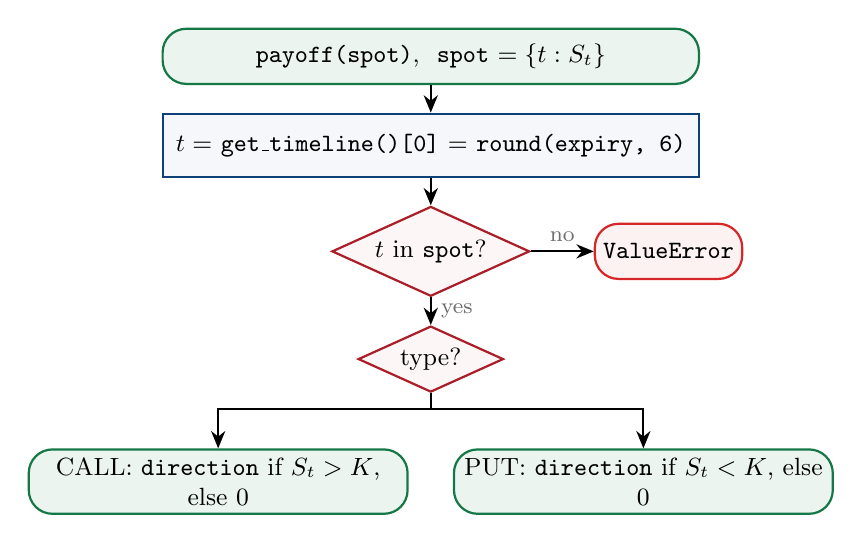
\begin{tikzpicture}[node distance=3.5mm]
\node[fcterm, text width=6.6cm] (in) {\texttt{payoff(spot)}, \ \texttt{spot} $=\{t: S_t\}$};
\node[fcbox, text width=6.6cm, below=of in] (t) {$t=$ \texttt{get\_timeline()[0]} $=$ \texttt{round(expiry, 6)}};
\node[fcdec, below=of t] (qk) {$t$ in \texttt{spot}?};
\node[fcerr, right=8mm of qk] (e) {\texttt{ValueError}};
\node[fcdec, below=of qk] (qy) {type?};
\node[fcterm, text width=4.6cm, below=7mm of qy, xshift=-2.7cm] (c) {CALL: \texttt{direction} if $S_t>K$, else $0$};
\node[fcterm, text width=4.6cm, below=7mm of qy, xshift=2.7cm] (p) {PUT: \texttt{direction} if $S_t<K$, else $0$};
\foreach \a/\b in {in/t,t/qk} \draw[fcarr] (\a) -- (\b);
\draw[fcarr] (qk) -- node[fclab, above] {no} (e);
\draw[fcarr] (qk) -- node[fclab, right] {yes} (qy);
\draw[fcarr] (qy.south) -- ++(0,-2mm) -| (c.north);
\draw[fcarr] (qy.south) -- ++(0,-2mm) -| (p.north);
\end{tikzpicture}
\captionof{figure}{Flowchart of \texttt{EuropeanDigitalContract.payoff}.}
\label{fig:payoff}
\end{minipage}\end{center}
\hwBlocks{1}{Q1 (a), \texttt{EuropeanDigitalContract}}

\step{Q1 (b): the pricer.} NEW VERSION of \texttt{EuropeanAnalyticPricer} (end of \texttt{pricer.py}). Change \#1: parent \texttt{Pricer}; change \#2: the type check asks for \texttt{EuropeanDigitalContract}; changes \#3--\#8: the fair value (Lemma 4) and the five Greeks (Lemma 5); the put uses $P_d=e^{-r\tau}-C_d$. $d_1,d_2$ are the static methods of the lecture's \texttt{EuropeanAnalyticPricer}.
\begin{lstlisting}[style=prof]
# =====================================================================================================
# Homework 3, Q1 (NEW CODE): NEW VERSION of EuropeanAnalyticPricer for EuropeanDigitalContract.
# Fair value (Lemma 4 of the report):  call  DF * N(d2),   put  DF * N(-d2) = DF - call   (DF = e^{-r tau})
# Greeks (Lemma 5): derivatives of DF * N(d2); the put follows from put = DF - call.
# d1, d2 are the static methods of EuropeanAnalyticPricer (reused, not copied).
# =====================================================================================================
# change # 1
#Delete.class EuropeanAnalyticPricer(Pricer):
# replace by
class EuropeanDigitalAnalyticPricer(Pricer):
# end change # 1
    # change # 2
    #Delete.def __init__(self, contract: EuropeanContract, model: MarketModel, params: Params) -> None:
    #Delete.    if not isinstance(contract, EuropeanContract):
    #Delete.        raise TypeError(f'Contract must be of type EuropeanContract but received {type(contract).__name__}')
    # replace by
    def __init__(self, contract: EuropeanDigitalContract, model: MarketModel, params: Params) -> None:
        if not isinstance(contract, EuropeanDigitalContract):
            raise TypeError(f'Contract must be of type EuropeanDigitalContract but received {type(contract).__name__}')
    # end change # 2
        super().__init__(contract, model, params)

    def calc_fair_value(self) -> float:
        direction = self.contract.direction
        strike = self.contract.strike
        expiry = self.contract.expiry
        time_to_expiry = expiry - self.valuation_time
        spot = self.model.spot
        vol = self.model.vol
        rate = self.model.risk_free_rate
        df = self.model.calc_df(time_to_expiry)
        # change # 3
        #Delete.d1 = EuropeanAnalyticPricer.calc_d1(spot / strike, vol, rate, time_to_expiry)
        d2 = EuropeanAnalyticPricer.calc_d2(spot / strike, vol, rate, time_to_expiry)
        #Delete.if self.contract.derivative_type == PutCallFwd.CALL:
        #Delete.    return direction * (spot * norm.cdf(d1) - strike * df * norm.cdf(d2))
        #Delete.elif self.contract.derivative_type == PutCallFwd.PUT:
        #Delete.    return direction * (strike * df * norm.cdf(-d2) - spot * norm.cdf(-d1))
        # replace by
        if self.contract.derivative_type == PutCallFwd.CALL:
            return direction * df * norm.cdf(d2)
        elif self.contract.derivative_type == PutCallFwd.PUT:
            return direction * df * norm.cdf(-d2)
        # end change # 3
        else:
            self.contract.raise_incorrect_derivative_type_error()

    def calc_delta(self) -> float:
        greek = 0.0
        spot = self.model.spot
        strike = self.contract.strike
        expiry = self.contract.expiry
        time_to_expiry = expiry - self.valuation_time
        vol = self.model.vol
        rate = self.model.risk_free_rate
        # change # 4
        #Delete.d1 = EuropeanAnalyticPricer.calc_d1(spot / strike, vol, rate, time_to_expiry)
        #Delete.if self.contract.derivative_type == PutCallFwd.CALL:
        #Delete.    greek = norm.cdf(d1)
        #Delete.elif self.contract.derivative_type == PutCallFwd.PUT:
        #Delete.    greek = -norm.cdf(-d1)
        # replace by
        df = self.model.calc_df(time_to_expiry)
        d2 = EuropeanAnalyticPricer.calc_d2(spot / strike, vol, rate, time_to_expiry)
        call_greek = df * norm.pdf(d2) / (spot * vol * np.sqrt(time_to_expiry))
        if self.contract.derivative_type == PutCallFwd.CALL:
            greek = call_greek
        elif self.contract.derivative_type == PutCallFwd.PUT:
            greek = -call_greek                                  # put = DF - call
        # end change # 4
        else:
            self.contract.raise_incorrect_derivative_type_error()
        return self.contract.direction * greek

    def calc_gamma(self) -> float:
        greek = 0.0
        spot = self.model.spot
        strike = self.contract.strike
        expiry = self.contract.expiry
        time_to_expiry = expiry - self.valuation_time
        vol = self.model.vol
        rate = self.model.risk_free_rate
        # change # 5
        #Delete.d1 = EuropeanAnalyticPricer.calc_d1(spot / strike, vol, rate, time_to_expiry)
        #Delete.if self.contract.derivative_type in (PutCallFwd.CALL, PutCallFwd.PUT):
        #Delete.    greek = norm.pdf(d1) / (spot * vol * np.sqrt(time_to_expiry))
        # replace by
        df = self.model.calc_df(time_to_expiry)
        d1 = EuropeanAnalyticPricer.calc_d1(spot / strike, vol, rate, time_to_expiry)
        d2 = EuropeanAnalyticPricer.calc_d2(spot / strike, vol, rate, time_to_expiry)
        call_greek = -df * norm.pdf(d2) * d1 / (spot**2 * vol**2 * time_to_expiry)
        if self.contract.derivative_type == PutCallFwd.CALL:
            greek = call_greek
        elif self.contract.derivative_type == PutCallFwd.PUT:
            greek = -call_greek
        # end change # 5
        else:
            self.contract.raise_incorrect_derivative_type_error()
        return self.contract.direction * greek

    def calc_vega(self) -> float:
        greek = 0.0
        spot = self.model.spot
        strike = self.contract.strike
        expiry = self.contract.expiry
        time_to_expiry = expiry - self.valuation_time
        vol = self.model.vol
        rate = self.model.risk_free_rate
        df = self.model.calc_df(time_to_expiry)
        # change # 6
        #Delete.d2 = EuropeanAnalyticPricer.calc_d2(spot / strike, vol, rate, time_to_expiry)
        #Delete.if self.contract.derivative_type in (PutCallFwd.CALL, PutCallFwd.PUT):
        #Delete.    greek = strike * df * norm.pdf(d2) * np.sqrt(time_to_expiry)
        # replace by
        d1 = EuropeanAnalyticPricer.calc_d1(spot / strike, vol, rate, time_to_expiry)
        d2 = EuropeanAnalyticPricer.calc_d2(spot / strike, vol, rate, time_to_expiry)
        call_greek = -df * norm.pdf(d2) * d1 / vol
        if self.contract.derivative_type == PutCallFwd.CALL:
            greek = call_greek
        elif self.contract.derivative_type == PutCallFwd.PUT:
            greek = -call_greek
        # end change # 6
        else:
            self.contract.raise_incorrect_derivative_type_error()
        return self.contract.direction * greek

    def calc_theta(self) -> float:
        greek = 0.0
        strike = self.contract.strike
        spot = self.model.spot
        expiry = self.contract.expiry
        time_to_expiry = expiry - self.valuation_time
        vol = self.model.vol
        rate = self.model.risk_free_rate
        df = self.model.calc_df(time_to_expiry)
        d1 = EuropeanAnalyticPricer.calc_d1(spot / strike, vol, rate, time_to_expiry)
        d2 = EuropeanAnalyticPricer.calc_d2(spot / strike, vol, rate, time_to_expiry)
        # change # 7
        #Delete.if self.contract.derivative_type == PutCallFwd.CALL:
        #Delete.    greek = -1.0 * ((spot * norm.pdf(d1) * vol) / (2 * np.sqrt(time_to_expiry))
        #Delete.                    + rate * strike * df * norm.cdf(d2))
        #Delete.elif self.contract.derivative_type == PutCallFwd.PUT:
        #Delete.    greek = -1.0 * ((spot * norm.pdf(d1) * vol) / (2 * np.sqrt(time_to_expiry))
        #Delete.                    - rate * strike * df * norm.cdf(-d2))
        # replace by
        call_greek = (rate * df * norm.cdf(d2)
                      + df * norm.pdf(d2) * (d1 / (2 * time_to_expiry) - rate / (vol * np.sqrt(time_to_expiry))))
        if self.contract.derivative_type == PutCallFwd.CALL:
            greek = call_greek
        elif self.contract.derivative_type == PutCallFwd.PUT:
            greek = rate * df - call_greek                       # theta of DF = e^{-r(T-t)} is r * DF
        # end change # 7
        else:
            self.contract.raise_incorrect_derivative_type_error()
        return self.contract.direction * greek

    def calc_rho(self) -> float:
        greek = 0.0
        strike = self.contract.strike
        expiry = self.contract.expiry
        time_to_expiry = expiry - self.valuation_time
        spot = self.model.spot
        vol = self.model.vol
        rate = self.model.risk_free_rate
        df = self.model.calc_df(time_to_expiry)
        d2 = EuropeanAnalyticPricer.calc_d2(spot / strike, vol, rate, time_to_expiry)
        # change # 8
        #Delete.if self.contract.derivative_type == PutCallFwd.CALL:
        #Delete.    greek = strike * time_to_expiry * df * norm.cdf(d2)
        #Delete.elif self.contract.derivative_type == PutCallFwd.PUT:
        #Delete.    greek = -strike * time_to_expiry * df * norm.cdf(-d2)
        # replace by
        call_greek = -time_to_expiry * df * norm.cdf(d2) + df * norm.pdf(d2) * np.sqrt(time_to_expiry) / vol
        if self.contract.derivative_type == PutCallFwd.CALL:
            greek = call_greek
        elif self.contract.derivative_type == PutCallFwd.PUT:
            greek = -time_to_expiry * df - call_greek            # rho of DF = e^{-r tau} is -tau * DF
        # end change # 8
        else:
            self.contract.raise_incorrect_derivative_type_error()
        return self.contract.direction * greek
\end{lstlisting}

\begin{center}\begin{minipage}{\linewidth}\centering
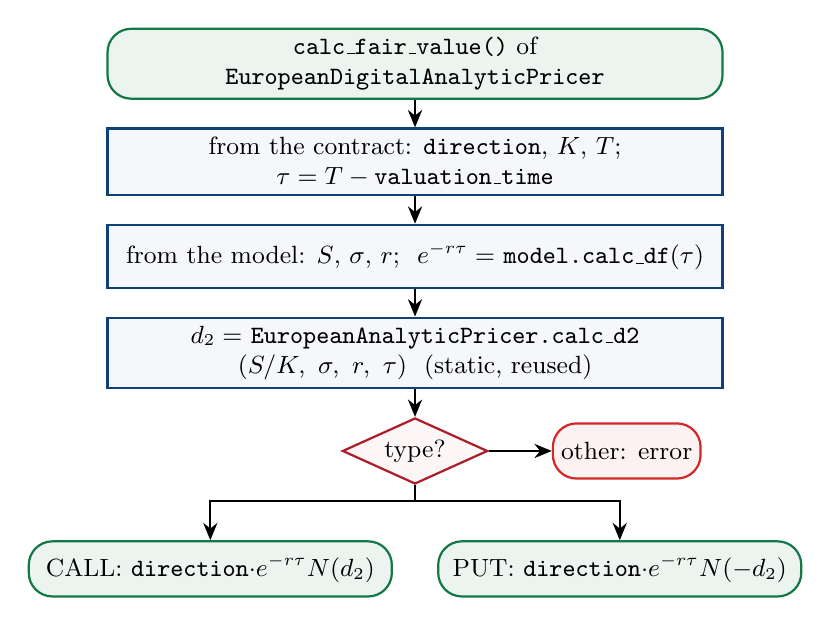
\begin{tikzpicture}[node distance=3.5mm]
\node[fcterm, text width=7.6cm] (i) {\texttt{calc\_fair\_value()} of \texttt{EuropeanDigitalAnalyticPricer}};
\node[fcbox, text width=7.6cm, below=of i] (c) {from the contract: \texttt{direction}, $K$, $T$; \ $\tau=T-\texttt{valuation\_time}$};
\node[fcbox, text width=7.6cm, below=of c] (m) {from the model: $S$, $\sigma$, $r$; \ $\DF=$ \texttt{model.calc\_df}$(\tau)$};
\node[fcbox, text width=7.6cm, below=of m] (d) {$d_2=$ \texttt{EuropeanAnalyticPricer.calc\_d2}\\ $(S/K,\ \sigma,\ r,\ \tau)$ \ (static, reused)};
\node[fcdec, below=of d] (t) {type?};
\node[fcterm, text width=4.4cm, below=7mm of t, xshift=-2.6cm] (cl) {CALL: \texttt{direction}$\cdot\DF N(d_2)$};
\node[fcterm, text width=4.4cm, below=7mm of t, xshift=2.6cm] (pu) {PUT: \texttt{direction}$\cdot\DF N(-d_2)$};
\node[fcerr, right=8mm of t] (er) {other: error};
\foreach \a/\b in {i/c,c/m,m/d,d/t} \draw[fcarr] (\a) -- (\b);
\draw[fcarr] (t.south) -- ++(0,-2mm) -| (cl.north);
\draw[fcarr] (t.south) -- ++(0,-2mm) -| (pu.north);
\draw[fcarr] (t) -- (er);
\end{tikzpicture}
\captionof{figure}{Flowchart of \texttt{calc\_fair\_value} of \texttt{EuropeanDigitalAnalyticPricer} (same skeleton as \texttt{EuropeanAnalyticPricer}, Lecture 5). The five Greeks follow the same steps with the formulas of Lemma 5.}
\label{fig:fv}
\end{minipage}\end{center}
\hwBlocks{2}{Q1 (b), \texttt{EuropeanDigitalAnalyticPricer}}

\step{Q1 (c): test of the new classes.} File \texttt{q1\_digital\_demo.py}: payoffs, fair values and parity (Lemma 4), the bull-spread bounds of the proof of Lemma 4 with the lecture's vanilla pricer, and the Greeks against bump and revaluation.
\begin{lstlisting}[style=pysmall]
# Homework 3, Q1: the digital option in the library (contract + analytic pricer), running example.
# Run from this folder with the course venv:  python q1_digital_demo.py   (printed output: q1_digital_demo.out)
import sys
from pathlib import Path

here = Path(__file__).resolve().parent
root = next((p for p in [here, *here.parents] if (p / 'src' / 'enums.py').exists()), here)
sys.path[:0] = [str(here), str(root)]               # this folder (library) and the repository (src.enums)

from pricer import *                                # library of Lecture 5 + the NEW classes (Homework 3)

# running example: the market of the library
model = MarketModel(Stock.BLUECHIP_BANK)
strike, expiry = 130.0, 1.0
print(f'market: S = {model.spot}, vol = {model.vol}, r = {model.risk_free_rate};  K = {strike}, T = {expiry}')

# 1. payoffs of the new contract (Definition 1)
long_call = EuropeanDigitalContract(Stock.BLUECHIP_BANK, PutCallFwd.CALL, LongShort.LONG, strike, expiry)
short_put = EuropeanDigitalContract(Stock.BLUECHIP_BANK, PutCallFwd.PUT, LongShort.SHORT, strike, expiry)
for s_T in [129.0, 131.0]:
    print(f'S_T = {s_T}: long digital call pays {long_call.payoff({expiry: s_T})}, '
          f'short digital put pays {short_put.payoff({expiry: s_T})}')

# 2. fair values (Lemma 4) and parity C_d + P_d = DF
pricers = {cp: EuropeanDigitalAnalyticPricer(
               EuropeanDigitalContract(Stock.BLUECHIP_BANK, cp, LongShort.LONG, strike, expiry), model, Params())
           for cp in (PutCallFwd.CALL, PutCallFwd.PUT)}
call, put = (pricers[cp].calc_fair_value() for cp in (PutCallFwd.CALL, PutCallFwd.PUT))
df = model.calc_df(expiry)
d2 = EuropeanAnalyticPricer.calc_d2(model.spot / strike, model.vol, model.risk_free_rate, expiry)
print(f'd2 = {d2:.6f}, DF = {df:.6f}')
print(f'digital call = {call:.6f}, digital put = {put:.6f}, call + put = {call + put:.6f} (DF = {df:.6f})')


# 3. bull spreads with the lecture's vanilla pricer (proof of Lemma 4)
def vanilla_call(k: float) -> float:
    contract = EuropeanContract(Stock.BLUECHIP_BANK, PutCallFwd.CALL, LongShort.LONG, k, expiry)
    return EuropeanAnalyticPricer(contract, model, Params()).calc_fair_value()


for h in [10.0, 1.0, 0.1, 0.01]:
    lower = (vanilla_call(strike) - vanilla_call(strike + h)) / h
    upper = (vanilla_call(strike - h) - vanilla_call(strike)) / h
    print(f'h = {h:5.2f}: {lower:.6f} <= C_d = {call:.6f} <= {upper:.6f}   {lower <= call <= upper}')

# 4. Greeks (Lemma 5) against bump and revaluation
print(f"{'':6s}{'call':>11s}{'put':>11s}{'call bump':>11s}")
pc = pricers[PutCallFwd.CALL]
hs, h = 0.01, 1e-4


def bumped(attribute: str, step: float) -> float:
    owner = pc if attribute == 'valuation_time' else model
    base = getattr(owner, attribute)
    setattr(owner, attribute, base + step)
    value = pc.calc_fair_value()
    setattr(owner, attribute, base)
    return value


bumps = {'delta': (bumped('spot', hs) - bumped('spot', -hs)) / (2 * hs),
         'gamma': (bumped('spot', hs) - 2 * call + bumped('spot', -hs)) / hs**2,
         'vega': (bumped('vol', h) - bumped('vol', -h)) / (2 * h),
         'theta': (bumped('valuation_time', h) - bumped('valuation_time', -h)) / (2 * h),
         'rho': (bumped('risk_free_rate', h) - bumped('risk_free_rate', -h)) / (2 * h)}
for g, b in bumps.items():
    gc = getattr(pricers[PutCallFwd.CALL], f'calc_{g}')()
    gp = getattr(pricers[PutCallFwd.PUT], f'calc_{g}')()
    print(f'{g:6s}{gc:11.6f}{gp:11.6f}{b:11.6f}')
\end{lstlisting}
\begin{lstlisting}[style=out]
market: S = 130.17, vol = 0.381, r = 0.05;  K = 130.0, T = 1.0
S_T = 129.0: long digital call pays 0.0, short digital put pays -1.0
S_T = 131.0: long digital call pays 1.0, short digital put pays 0.0
d2 = -0.055836, DF = 0.951229
digital call = 0.454437, digital put = 0.496793, call + put = 0.951229 (DF = 0.951229)
h = 10.00: 0.417385 <= C_d = 0.454437 <= 0.493716   True
h =  1.00: 0.450623 <= C_d = 0.454437 <= 0.458273   True
h =  0.10: 0.454054 <= C_d = 0.454437 <= 0.454819   True
h =  0.01: 0.454398 <= C_d = 0.454437 <= 0.454475   True
             call        put  call bump
delta    0.007640  -0.007640   0.007640
gamma   -0.000050   0.000050  -0.000050
vega    -0.323367   0.323367  -0.323367
theta    0.034599   0.012962   0.034599
rho      0.540037  -1.491267   0.540037
\end{lstlisting}
\noindent Reading: $C_d=0.454437$ and $P_d=0.496793$ add up to $e^{-0.05}=0.951229$ (Lemma 4); every bull-spread pair brackets $C_d$ and the bracket shrinks with $h$ (proof of Lemma 4); each Greek equals its bump (Lemma 5); the put's Greeks are those of $e^{-r\tau}-C_d$.

\step{Q1 (d): the unit tests.} End of \texttt{test\_pricer.py}, after the professor's \texttt{TestPutCallParity}. The fair value is tested in \texttt{TestDigitalFairValue} on the grid of the lecture (2 stocks $\times$ 3 values of $K/S$ $\times$ 4 expiries) and in \texttt{test\_digital\_value\_by\_hand}; the payoff, the type checks and the Greeks have their own tests.
\begin{lstlisting}[style=pysmall]
# =====================================================================================================
# Homework 3, Q1 (NEW CODE): unit tests of the digital option.
# Fair value (asked in the assignment) + payoff, type checks and Greeks.
# =====================================================================================================
def digital_pricer(model: MarketModel, call_put: PutCallFwd, long_short: LongShort, strike: float,
                   expiry: float) -> EuropeanDigitalAnalyticPricer:
    contract = EuropeanDigitalContract(model.underlying, call_put, long_short, strike, expiry)
    return EuropeanDigitalAnalyticPricer(contract, model, Params())


def call_price(model: MarketModel, strike: float, expiry: float) -> float:
    """Long vanilla call of the lecture (EuropeanAnalyticPricer)."""
    contract = EuropeanContract(model.underlying, PutCallFwd.CALL, LongShort.LONG, strike, expiry)
    return EuropeanAnalyticPricer(contract, model, Params()).calc_fair_value()


@pytest.mark.parametrize('underlying', [Stock.BLUECHIP_BANK, Stock.TIPTOP_SOLUTIONS])
@pytest.mark.parametrize('strike_over_spot', np.arange(0.5, 2.0, 0.5))
@pytest.mark.parametrize('expiry', np.arange(0.5, 2.5, 0.5))
class TestDigitalFairValue:
    def test_digital_parity(self, underlying, strike_over_spot, expiry):
        # long digital call + long digital put pay 1 at T, worth DF = e^{-rT} today (Lemma 4)
        model = MarketModel(underlying)
        strike = strike_over_spot * model.spot
        call = digital_pricer(model, PutCallFwd.CALL, LongShort.LONG, strike, expiry).calc_fair_value()
        put = digital_pricer(model, PutCallFwd.PUT, LongShort.LONG, strike, expiry).calc_fair_value()
        assert call + put == pytest.approx(model.calc_df(expiry), abs=1e-12)

    def test_bull_spread_bounds(self, underlying, strike_over_spot, expiry):
        # (c(K) - c(K+h))/h <= C_d <= (c(K-h) - c(K))/h for every h > 0 (proof of Lemma 4); h = 1% of K
        model = MarketModel(underlying)
        strike = strike_over_spot * model.spot
        h = 0.01 * strike
        digital = digital_pricer(model, PutCallFwd.CALL, LongShort.LONG, strike, expiry).calc_fair_value()
        lower = (call_price(model, strike, expiry) - call_price(model, strike + h, expiry)) / h
        upper = (call_price(model, strike - h, expiry) - call_price(model, strike, expiry)) / h
        assert lower <= digital <= upper

    def test_bull_spread_limit(self, underlying, strike_over_spot, expiry):
        # a narrow scaled bull spread (width h = 0.01% of K) has the price of the digital call (Lemma 4)
        model = MarketModel(underlying)
        strike = strike_over_spot * model.spot
        h = 1e-4 * strike
        digital = digital_pricer(model, PutCallFwd.CALL, LongShort.LONG, strike, expiry).calc_fair_value()
        spread = (call_price(model, strike - h / 2, expiry) - call_price(model, strike + h / 2, expiry)) / h
        assert spread == pytest.approx(digital, abs=1e-6)

    def test_short_is_minus_long(self, underlying, strike_over_spot, expiry):
        model = MarketModel(underlying)
        strike = strike_over_spot * model.spot
        for call_put in (PutCallFwd.CALL, PutCallFwd.PUT):
            long = digital_pricer(model, call_put, LongShort.LONG, strike, expiry).calc_fair_value()
            short = digital_pricer(model, call_put, LongShort.SHORT, strike, expiry).calc_fair_value()
            assert short == pytest.approx(-long, abs=1e-15)


def test_digital_value_by_hand():
    # BLUECHIP_BANK (S = 130.17, vol = 0.381, r = 0.05), K = 130, T = 1:
    # d2 = -0.055836, DF = 0.951229, C_d = DF * N(d2) = 0.454437, P_d = DF * N(-d2) = 0.496793
    model = MarketModel(Stock.BLUECHIP_BANK)
    call = digital_pricer(model, PutCallFwd.CALL, LongShort.LONG, 130.0, 1.0).calc_fair_value()
    put = digital_pricer(model, PutCallFwd.PUT, LongShort.LONG, 130.0, 1.0).calc_fair_value()
    assert call == pytest.approx(0.454437, abs=1e-6)
    assert put == pytest.approx(0.496793, abs=1e-6)


def test_digital_payoff():
    long_call = EuropeanDigitalContract(Stock.BLUECHIP_BANK, PutCallFwd.CALL, LongShort.LONG, 130.0, 1.0)
    short_put = EuropeanDigitalContract(Stock.BLUECHIP_BANK, PutCallFwd.PUT, LongShort.SHORT, 130.0, 1.0)
    assert long_call.payoff({1.0: 131.0}) == 1.0
    assert long_call.payoff({1.0: 129.0}) == 0.0
    assert short_put.payoff({1.0: 129.0}) == -1.0
    assert short_put.payoff({1.0: 131.0}) == 0.0
    with pytest.raises(ValueError):
        long_call.payoff({0.5: 131.0})                 # no spot at the expiry


def test_digital_type_checks():
    model = MarketModel(Stock.BLUECHIP_BANK)
    vanilla = EuropeanContract(Stock.BLUECHIP_BANK, PutCallFwd.CALL, LongShort.LONG, 130.0, 1.0)
    digital = EuropeanDigitalContract(Stock.BLUECHIP_BANK, PutCallFwd.CALL, LongShort.LONG, 130.0, 1.0)
    with pytest.raises(ValueError):
        EuropeanDigitalContract(Stock.BLUECHIP_BANK, PutCallFwd.FWD, LongShort.LONG, 130.0, 1.0)
    with pytest.raises(TypeError):
        EuropeanDigitalAnalyticPricer(vanilla, model, Params())      # a vanilla is not a digital
    with pytest.raises(TypeError):
        EuropeanAnalyticPricer(digital, model, Params())             # the vanilla pricer rejects a digital


def bumped_value(pricer: EuropeanDigitalAnalyticPricer, attribute: str, h: float) -> float:
    """Fair value after adding h to the model's spot / vol / risk_free_rate, or to the valuation time."""
    owner = pricer if attribute == 'valuation_time' else pricer.model
    base = getattr(owner, attribute)
    setattr(owner, attribute, base + h)
    value = pricer.calc_fair_value()
    setattr(owner, attribute, base)
    return value


@pytest.mark.parametrize('call_put', [PutCallFwd.CALL, PutCallFwd.PUT])
@pytest.mark.parametrize('long_short', [LongShort.LONG, LongShort.SHORT])
def test_digital_greeks_bump(call_put, long_short):
    # analytic Greeks (Lemma 5) = central differences of the fair value
    pricer = digital_pricer(MarketModel(Stock.BLUECHIP_BANK), call_put, long_short, 130.0, 1.0)
    fv = pricer.calc_fair_value()
    hs, h = 0.01, 1e-4
    bump = {
        'delta': (bumped_value(pricer, 'spot', hs) - bumped_value(pricer, 'spot', -hs)) / (2 * hs),
        'gamma': (bumped_value(pricer, 'spot', hs) - 2 * fv + bumped_value(pricer, 'spot', -hs)) / hs**2,
        'vega': (bumped_value(pricer, 'vol', h) - bumped_value(pricer, 'vol', -h)) / (2 * h),
        'theta': (bumped_value(pricer, 'valuation_time', h) - bumped_value(pricer, 'valuation_time', -h)) / (2 * h),
        'rho': (bumped_value(pricer, 'risk_free_rate', h) - bumped_value(pricer, 'risk_free_rate', -h)) / (2 * h)}
    analytic = {'delta': pricer.calc_delta(), 'gamma': pricer.calc_gamma(), 'vega': pricer.calc_vega(),
                'theta': pricer.calc_theta(), 'rho': pricer.calc_rho()}
    assert analytic == pytest.approx(bump, rel=1e-4, abs=1e-8)
\end{lstlisting}

\begin{center}\begin{minipage}{\linewidth}\centering
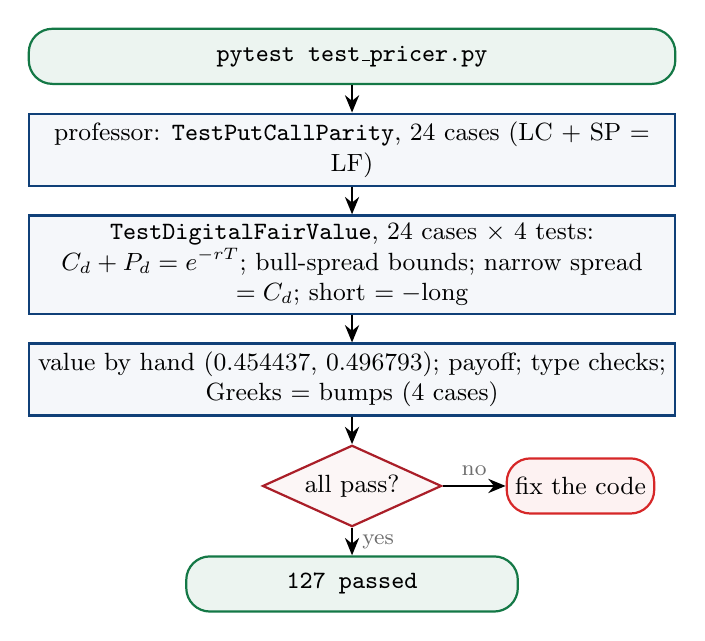
\begin{tikzpicture}[node distance=3.5mm]
\node[fcterm, text width=8cm] (s) {\texttt{pytest test\_pricer.py}};
\node[fcbox, text width=8cm, below=of s] (a) {professor: \texttt{TestPutCallParity}, 24 cases (LC $+$ SP $=$ LF)};
\node[fcbox, text width=8cm, below=of a] (b) {\texttt{TestDigitalFairValue}, 24 cases $\times$ 4 tests: $C_d+P_d=e^{-rT}$; bull-spread bounds; narrow spread $=C_d$; short $=-$long};
\node[fcbox, text width=8cm, below=of b] (c) {value by hand ($0.454437$, $0.496793$); payoff; type checks; Greeks $=$ bumps (4 cases)};
\node[fcdec, below=of c] (q) {all pass?};
\node[fcerr, right=8mm of q] (f) {fix the code};
\node[fcterm, text width=4cm, below=of q] (ok) {\texttt{127 passed}};
\foreach \x/\y in {s/a,a/b,b/c,c/q} \draw[fcarr] (\x) -- (\y);
\draw[fcarr] (q) -- node[fclab, above] {no} (f);
\draw[fcarr] (q) -- node[fclab, right] {yes} (ok);
\end{tikzpicture}
\captionof{figure}{Flowchart of the unit tests.}
\label{fig:tests}
\end{minipage}\end{center}

\noindent Run from the repository folder, and output:
\begin{lstlisting}[style=out]
python -m pytest -q homeworks/54932fw/3_HW_LECTURE_5/test_pricer.py
\end{lstlisting}
\begin{lstlisting}[style=out]
........................................................................ [ 56%]
.......................................................                  [100%]
127 passed in 0.85s
\end{lstlisting}
\hwBlocks{3}{Q1 (d), the unit tests}

\ansbox{\textbf{Q1.} \texttt{EuropeanDigitalContract} pays \texttt{direction} $\cdot\,\ind\{S_T>K\}$ (call) or \texttt{direction} $\cdot\,\ind\{S_T<K\}$ (put); \texttt{EuropeanDigitalAnalyticPricer} returns $C_d=e^{-r\tau}N(d_2)$, $P_d=e^{-r\tau}N(-d_2)$ and the five Greeks of Lemma 5, times \texttt{direction}. All 127 unit tests pass (the professor's 24 and 103 new ones). Running example: $C_d=0.454437$, $P_d=0.496793$.}


% =====================================================================
\subhead{5. Q2: the digital call as a limit of bull call spreads.}
\emph{Get familiar with bull spread options and by utilizing EuropeanDigitalAnalyticPricer and EuropeanAnalyticPricer, create a figure to visualize that a digital call option can be thought of as a limit of bull spread call options.}

\noindent\textbf{Idea} (the proof of Lemma 4 as a picture). A bull spread of width $h$ (Definition~2) is a LONG call with strike $K$ and a SHORT call with strike $K+h$; it pays at most $h$, so we hold $1/h$ of it. Its payoff tends to $\ind\{S_T>K\}$ as $h\to0$, and its price $R_h=\frac{c(K)-c(K+h)}{h}$ tends to $C_d$ (Lemma 4). The left spread $L_h=\frac{c(K-h)-c(K)}{h}$ approaches $C_d$ from above. In the library a spread is two \texttt{EuropeanAnalyticPricer}s, the second with \texttt{LongShort.SHORT}: its \texttt{direction} $=-1$ makes the sum of the two fair values the price of the spread. The digital is priced with \texttt{EuropeanDigitalAnalyticPricer} (Q1). The figure has three panels: (a) payoffs at $T$, (b) prices today against the spot, (c) the error against $h$.

\step{Q2 (a): the code} (file \texttt{q2\_bull\_spread.py}; the plots use \texttt{my\_plotter} of Homework~1, file \texttt{plotter.py}).
\begin{lstlisting}[style=pysmall]
# Homework 3, Q2: a digital call is the limit of (scaled) bull call spreads.
# Uses EuropeanAnalyticPricer (lecture) for the spreads and EuropeanDigitalAnalyticPricer (Q1) for the digital;
# the plots are drawn with my_plotter of Homework 1 (plotter.py).
# Run from this folder with the course venv:  python q2_bull_spread.py   (output: q2_bull_spread.out, figures/)
import sys
from pathlib import Path

here = Path(__file__).resolve().parent
root = next((p for p in [here, *here.parents] if (p / 'src' / 'enums.py').exists()), here)
sys.path[:0] = [str(here), str(root)]               # this folder (library) and the repository (src.enums)

import matplotlib
matplotlib.use('Agg')                                # files only (no window)
import matplotlib.pyplot as plt
import numpy as np
from pricer import *                                 # library of Lecture 5 + the classes of Q1
from plotter import my_plotter                       # Homework 1 (HW 2/1)

stock, strike, expiry = Stock.BLUECHIP_BANK, 130.0, 1.0
model = MarketModel(stock)


def bull_spread(k_low: float, k_high: float) -> list[EuropeanAnalyticPricer]:
    """Bull call spread (Definition 2): LONG call with strike k_low + SHORT call with strike k_high."""
    long_leg = EuropeanContract(stock, PutCallFwd.CALL, LongShort.LONG, k_low, expiry)
    short_leg = EuropeanContract(stock, PutCallFwd.CALL, LongShort.SHORT, k_high, expiry)
    return [EuropeanAnalyticPricer(long_leg, model, Params()), EuropeanAnalyticPricer(short_leg, model, Params())]


def scaled_value(legs: list[EuropeanAnalyticPricer], h: float) -> float:
    """Price of (1/h) x bull spread: the sum of the two legs (the SHORT leg is negative), divided by h."""
    return sum(leg.calc_fair_value() for leg in legs) / h


def scaled_payoff(legs: list[EuropeanAnalyticPricer], h: float, s_T: float) -> float:
    return sum(leg.contract.payoff({expiry: s_T}) for leg in legs) / h


def at_spot(pricer_value, s: float) -> float:
    """Value with the model's spot set to s (the model is shared by all pricers), then restore it."""
    base = model.spot
    model.spot = s
    value = pricer_value()
    model.spot = base
    return value


digital_contract = EuropeanDigitalContract(stock, PutCallFwd.CALL, LongShort.LONG, strike, expiry)
digital = EuropeanDigitalAnalyticPricer(digital_contract, model, Params())
c_d = digital.calc_fair_value()
print(f'market: S = {model.spot}, vol = {model.vol}, r = {model.risk_free_rate};  K = {strike}, T = {expiry}')
print(f'digital call C_d = {c_d:.6f}')

# 1. table: right spread R_h = (1/h)(K, K+h) <= C_d <= left spread L_h = (1/h)(K-h, K)  (proof of Lemma 4)
print(f"{'h':>7s}{'R_h':>11s}{'L_h':>11s}{'C_d - R_h':>12s}{'L_h - C_d':>12s}")
widths = np.array([40.0, 20.0, 10.0, 5.0, 2.0, 1.0, 0.5, 0.1, 0.01])
right = np.array([scaled_value(bull_spread(strike, strike + h), h) for h in widths])
left = np.array([scaled_value(bull_spread(strike - h, strike), h) for h in widths])
for h, r_h, l_h in zip(widths, right, left):
    print(f'{h:7.2f}{r_h:11.6f}{l_h:11.6f}{c_d - r_h:12.2e}{l_h - c_d:12.2e}')
slope = np.polyfit(np.log(widths[-4:]), np.log(c_d - right[-4:]), 1)[0]
print(f'error of R_h ~ h^{slope:.2f} for small h (first order)')

# 2. figure: (a) payoffs at T, (b) prices today against the spot, (c) price error against h
plot_widths = [20.0, 10.0, 2.0]
colors = ['tab:green', 'tab:orange', 'tab:blue', 'black']
names = [f'bull spread / h, h = {h:g}' for h in plot_widths] + ['digital call']
fig, axes = plt.subplots(1, 3, figsize=(18, 5))

s_T = np.linspace(100.0, 160.0, 601)
payoffs = [[scaled_payoff(bull_spread(strike, strike + h), h, s) for s in s_T] for h in plot_widths]
payoffs.append([digital.contract.payoff({expiry: s}) for s in s_T])
my_plotter(s_T, payoffs, names=names, ax=axes[0],
           layout={'title': '(a) payoff at expiry', 'x_label': '$S_T$', 'y_label': 'payoff',
                   'colors': colors, 'linestyles': ['-', '-', '-', '--'], 'linewidth': 2, 'title_fontsize': 14,
                   'label_fontsize': 12, 'legend_fontsize': 10, 'title_pad': 10, 'label_pad': 5,
                   'hline': None, 'vlines': [strike], 'grid': True, 'legend_loc': 'upper left'})

spots = np.linspace(60.0, 220.0, 161)
prices = [[at_spot(lambda: scaled_value(bull_spread(strike, strike + h), h), s) for s in spots] for h in plot_widths]
prices.append([at_spot(digital.calc_fair_value, s) for s in spots])
my_plotter(spots, prices, names=names, ax=axes[1],
           layout={'title': '(b) price today', 'x_label': 'spot $S$', 'y_label': 'price',
                   'colors': colors, 'linestyles': ['-', '-', '-', '--'], 'linewidth': 2, 'title_fontsize': 14,
                   'label_fontsize': 12, 'legend_fontsize': 10, 'title_pad': 10, 'label_pad': 5,
                   'hline': None, 'vlines': [strike], 'grid': True, 'legend_loc': 'upper left'})

my_plotter(widths, [c_d - right, left - c_d], names=['$C_d - R_h$ (right spread)', '$L_h - C_d$ (left spread)'],
           ax=axes[2],
           layout={'title': '(c) error against the width h', 'x_label': 'h (log scale)',
                   'y_label': 'error (log scale)', 'colors': ['tab:blue', 'tab:red'], 'markers': ['o', 's'],
                   'linewidth': 2, 'title_fontsize': 14, 'label_fontsize': 12, 'legend_fontsize': 10,
                   'title_pad': 10, 'label_pad': 5, 'hline': None, 'logx': True, 'logy': True, 'grid': True,
                   'legend_loc': 'upper left'})
fig.suptitle(f'Digital call = limit of bull call spreads  (BLUECHIP_BANK, K = {strike:g}, T = {expiry:g},'
             f' C_d = {c_d:.4f})', fontsize=15)
fig.tight_layout()
(here / 'figures').mkdir(exist_ok=True)
fig.savefig(here / 'figures' / 'q2_digital_vs_bull_spreads.pdf')
fig.savefig(here / 'figures' / 'q2_digital_vs_bull_spreads.png', dpi=110)
print('figure saved: figures/q2_digital_vs_bull_spreads.pdf (and .png)')
\end{lstlisting}
\begin{lstlisting}[style=out]
market: S = 130.17, vol = 0.381, r = 0.05;  K = 130.0, T = 1.0
digital call C_d = 0.454437
      h        R_h        L_h   C_d - R_h   L_h - C_d
  40.00   0.322478   0.617161    1.32e-01    1.63e-01
  20.00   0.382947   0.534585    7.15e-02    8.01e-02
  10.00   0.417385   0.493716    3.71e-02    3.93e-02
   5.00   0.435603   0.473831    1.88e-02    1.94e-02
   2.00   0.446832   0.462131    7.60e-03    7.69e-03
   1.00   0.450623   0.458273    3.81e-03    3.84e-03
   0.50   0.452527   0.456352    1.91e-03    1.92e-03
   0.10   0.454054   0.454819    3.82e-04    3.83e-04
   0.01   0.454398   0.454475    3.82e-05    3.83e-05
error of R_h ~ h^1.00 for small h (first order)
figure saved: figures/q2_digital_vs_bull_spreads.pdf (and .png)
\end{lstlisting}

\begin{center}\begin{minipage}{\linewidth}\centering
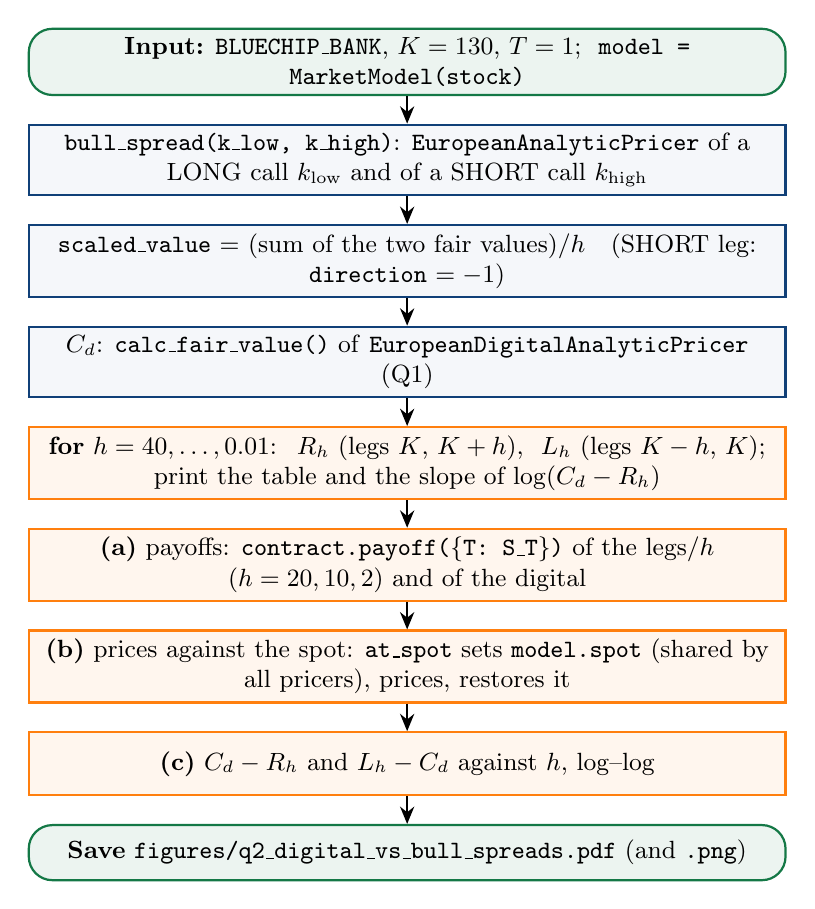
\begin{tikzpicture}[node distance=3.5mm]
\node[fcterm, text width=9.4cm] (in) {\textbf{Input:} \texttt{BLUECHIP\_BANK}, $K=130$, $T=1$; \ \texttt{model = MarketModel(stock)}};
\node[fcbox, text width=9.4cm, below=of in] (bs) {\texttt{bull\_spread(k\_low, k\_high)}: \texttt{EuropeanAnalyticPricer} of a LONG call $k_{\text{low}}$ and of a SHORT call $k_{\text{high}}$};
\node[fcbox, text width=9.4cm, below=of bs] (sv) {\texttt{scaled\_value} $=$ (sum of the two fair values)$/h$ \ \ (SHORT leg: \texttt{direction} $=-1$)};
\node[fcbox, text width=9.4cm, below=of sv] (cd) {$C_d$: \texttt{calc\_fair\_value()} of \texttt{EuropeanDigitalAnalyticPricer} (Q1)};
\node[fcplot, text width=9.4cm, below=of cd] (loop) {\textbf{for} $h=40,\dots,0.01$: \ $R_h$ (legs $K$, $K+h$), \ $L_h$ (legs $K-h$, $K$); print the table and the slope of $\log(C_d-R_h)$};
\node[fcplot, text width=9.4cm, below=of loop] (fa) {\textbf{(a)} payoffs: \texttt{contract.payoff(\{T: S\_T\})} of the legs$/h$ ($h=20,10,2$) and of the digital};
\node[fcplot, text width=9.4cm, below=of fa] (fb) {\textbf{(b)} prices against the spot: \texttt{at\_spot} sets \texttt{model.spot} (shared by all pricers), prices, restores it};
\node[fcplot, text width=9.4cm, below=of fb] (fc) {\textbf{(c)} $C_d-R_h$ and $L_h-C_d$ against $h$, log--log};
\node[fcterm, text width=9.4cm, below=of fc] (out) {\textbf{Save} \texttt{figures/q2\_digital\_vs\_bull\_spreads.pdf} (and \texttt{.png})};
\foreach \a/\b in {in/bs,bs/sv,sv/cd,cd/loop,loop/fa,fa/fb,fb/fc,fc/out} \draw[fcarr] (\a) -- (\b);
\end{tikzpicture}
\captionof{figure}{Flowchart of \texttt{q2\_bull\_spread.py}.}
\label{fig:q2flow}
\end{minipage}\end{center}

\step{Q2 (b): the figure} (drawn here with the same numbers as the figure the script saves in \texttt{figures/}).
\begin{center}\begin{minipage}{\linewidth}\centering
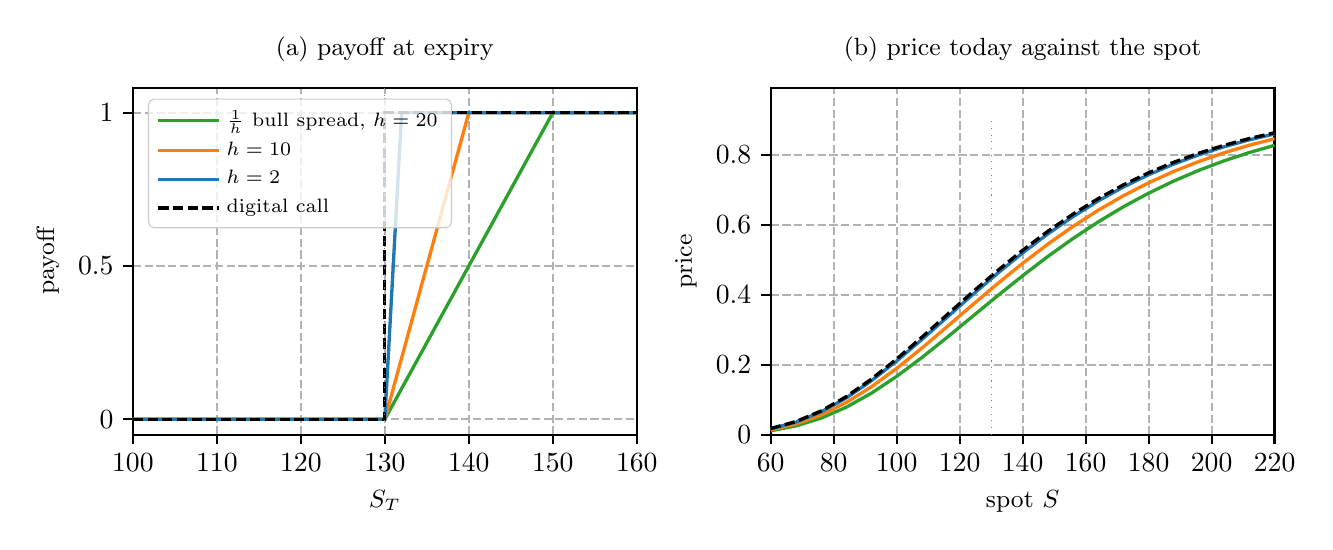
\begin{tikzpicture}
\begin{axis}[mpl, mplgrid, width=6.4cm, height=4.4cm, title={(a) payoff at expiry}, xlabel={$S_T$}, ylabel={payoff},
  xmin=100, xmax=160, ymin=-0.05, ymax=1.08, legend pos=north west, legend style={font=\scriptsize},
  title style={font=\small}, label style={font=\small}]
\addplot[tabgreen, line width=1.2pt] coordinates {(100,0) (130,0) (150,1) (160,1)}; \addlegendentry{$\frac1h$ bull spread, $h=20$}
\addplot[taborange, line width=1.2pt] coordinates {(100,0) (130,0) (140,1) (160,1)}; \addlegendentry{$h=10$}
\addplot[tabblue, line width=1.2pt] coordinates {(100,0) (130,0) (132,1) (160,1)}; \addlegendentry{$h=2$}
\addplot[black, line width=1.2pt, mpldash] coordinates {(100,0) (130,0) (130,1) (160,1)}; \addlegendentry{digital call}
\addplot[black!50, dotted] coordinates {(130,-0.05) (130,1.08)};
\end{axis}
\begin{axis}[mpl, mplgrid, at={(8.1cm,0)}, width=6.4cm, height=4.4cm, title={(b) price today against the spot}, xlabel={spot $S$}, ylabel={price},
  xmin=60, xmax=220, ymin=0, title style={font=\small}, label style={font=\small}]
\addplot[tabgreen, line width=1.2pt] coordinates {(60,0.01111) (68,0.02485) (76,0.04698) (84,0.07831) (92,0.11853) (100,0.16644) (108,0.22023) (116,0.27781) (124,0.33715) (132,0.39641) (140,0.45411) (148,0.50908) (156,0.56053) (164,0.60797) (172,0.65115) (180,0.69005) (188,0.72477) (196,0.75552) (204,0.78257) (212,0.80623) (220,0.82682)};
\addplot[taborange, line width=1.2pt] coordinates {(60,0.01379) (68,0.03020) (76,0.05602) (84,0.09177) (92,0.13676) (100,0.18934) (108,0.24732) (116,0.30836) (124,0.37026) (132,0.43114) (140,0.48955) (148,0.54443) (156,0.59512) (164,0.64126) (172,0.68275) (180,0.71967) (188,0.75225) (196,0.78078) (204,0.80561) (212,0.82711) (220,0.84563)};
\addplot[tabblue, line width=1.2pt] coordinates {(60,0.01664) (68,0.03570) (76,0.06502) (84,0.10482) (92,0.15399) (100,0.21048) (108,0.27178) (116,0.33537) (124,0.39897) (132,0.46071) (140,0.51922) (148,0.57354) (156,0.62316) (164,0.66784) (172,0.70762) (180,0.74267) (188,0.77331) (196,0.79990) (204,0.82284) (212,0.84254) (220,0.85937)};
\addplot[black, line width=1.2pt, mpldash] coordinates {(60,0.01747) (68,0.03728) (76,0.06756) (84,0.10844) (92,0.15870) (100,0.21618) (108,0.27830) (116,0.34249) (124,0.40645) (132,0.46833) (140,0.52678) (148,0.58090) (156,0.63018) (164,0.67444) (172,0.71374) (180,0.74829) (188,0.77841) (196,0.80450) (204,0.82696) (212,0.84620) (220,0.86261)};
\addplot[black!50, dotted] coordinates {(130,0) (130,0.9)};
\end{axis}
\end{tikzpicture}

\vspace{3mm}
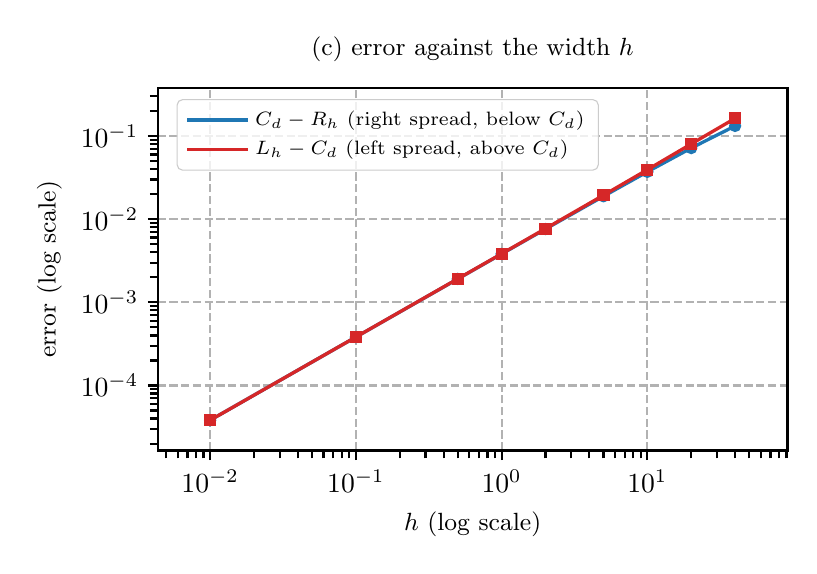
\begin{tikzpicture}
\begin{axis}[mpl, mplgrid, xmode=log, ymode=log, width=8cm, height=4.6cm, title={(c) error against the width $h$}, xlabel={$h$ (log scale)},
  ylabel={error (log scale)}, legend pos=north west, legend style={font=\scriptsize}, title style={font=\small}, label style={font=\small}]
\addplot[tabblue, line width=1.2pt, mark=*, mark size=1.6pt] coordinates {(40,1.3196e-01) (20,7.1489e-02) (10,3.7051e-02) (5,1.8834e-02) (2,7.6042e-03) (1,3.8136e-03) (0.5,1.9096e-03) (0.1,3.8238e-04) (0.01,3.8248e-05)}; \addlegendentry{$C_d-R_h$ (right spread, below $C_d$)}
\addplot[tabred, line width=1.2pt, mark=square*, mark size=1.6pt] coordinates {(40,1.6272e-01) (20,8.0148e-02) (10,3.9279e-02) (5,1.9395e-02) (2,7.6941e-03) (1,3.8361e-03) (0.5,1.9153e-03) (0.1,3.8260e-04) (0.01,3.8250e-05)}; \addlegendentry{$L_h-C_d$ (left spread, above $C_d$)}
\end{axis}
\end{tikzpicture}
\captionof{figure}{The digital call as a limit of bull call spreads (\texttt{BLUECHIP\_BANK}, $K=130$, $T=1$, $C_d=0.4544$). (a) The payoff of $\frac1h$ bull spread differs from the digital only on $(K,K+h)$. (b) For every spot the prices of the scaled spreads ($h=20,10,2$, \texttt{EuropeanAnalyticPricer}) approach the digital price (dashed, \texttt{EuropeanDigitalAnalyticPricer}). (c) Both errors go to $0$ like $h$.}
\label{fig:q2}
\end{minipage}\end{center}

\noindent Reading: in (a) the ramp of width $h$ becomes the step of the digital; in (b) the curve for $h=2$ is already on top of the digital curve; in (c) the right spreads stay below $C_d$ and the left spreads above it (the sandwich of the proof of Lemma 4), and both errors decrease like $h$ (slope $1.00$ in the output; e.g.\ $h=0.01$: $3.8\times10^{-5}$).

\hwBlocks{4}{Q2, \texttt{q2\_bull\_spread.py}: all blocks of the homework}

\ansbox{\textbf{Q2.} A digital call is the limit of $\frac1h$ bull call spreads (LONG call $K$, SHORT call $K+h$): the payoffs tend to $\ind\{S_T>K\}$, and the prices, computed with \texttt{EuropeanAnalyticPricer}, tend to the price of \texttt{EuropeanDigitalAnalyticPricer}, $C_d=e^{-r\tau}N(d_2)$, for every spot (Figure~\ref{fig:q2}). Running example: $R_{0.01}=0.454398<C_d=0.454437<L_{0.01}=0.454475$.}

\subhead{Comment (to keep in mind).}
\begin{itemize}
\item \emph{Other routes to Lemma 4.} The formula is also the risk-neutral value $e^{-r\tau}\,\Q(S_T>K)$, with $S_T$ log-normal under $\Q$; continuous-time risk-neutral pricing is not presented in the lectures (only its tree version, Lecture 4), see [5]. And $f=e^{-r\tau}N(d_2)$ satisfies the Black--Scholes PDE of Theorem 2 with $f\to\ind\{S>K\}$ as $\tau\to0$ (checked numerically: residual $\approx10^{-10}$).
\item \emph{One-sided and centred spreads.} $R_h$ and $L_h$ have error of order $h$ (panel (c)); their average, the centred spread $\frac{c(K-h/2)-c(K+h/2)}{h}$, has error of order $h^2$, which is why the unit test \texttt{test\_bull\_spread\_limit} uses it with a small tolerance.
\item \emph{Lecture code.} \texttt{EuropeanContract(..., FWD, ...)} raises \texttt{AttributeError} instead of the intended \texttt{ValueError}; the new contract stores the type first (change \#2).
\end{itemize}

\subhead{References.}
\begin{enumerate}[label={[\arabic*]}]
\item Lecture 3 of this course: \texttt{presentation\_03\_option\_basics\_and\_bsm\_model\_2026.ipynb} (forwards, calls, puts, parity, Black--Scholes PDE and formula, Greeks).
\item Lecture 5 of this course: \texttt{notebook\_building\_blocks.ipynb} and the \texttt{solution} folder (the library).
\item Lecture 4 of this course: \texttt{Tree.ipynb} (risk-neutral pricing in the tree; literature: Shreve I).
\item J.~C.~Hull, \emph{Options, Futures, and Other Derivatives}, Pearson: chapter ``Trading Strategies Involving Options'' (bull spreads) and chapter ``Exotic Options'' (binary options: cash-or-nothing call $Q\,e^{-rT}N(d_2)$).
\item S.~E.~Shreve, \emph{Stochastic Calculus for Finance II: Continuous-Time Models}, Springer, 2004, Ch.~5 (risk-neutral pricing); and Vol.~I, Ch.~1 (no arbitrage), the literature of Lecture 4.
\item D.~T.~Breeden, R.~H.~Litzenberger, Prices of state-contingent claims implicit in option prices, \emph{Journal of Business} 51(4), 1978, 621--651 (the strike derivative of the call price as the price of a digital).
\end{enumerate}

\end{document}
